
%% bare_conf.tex
%% V1.4b
%% 2015/08/26
%% by Michael Shell
%% See:
%% http://www.michaelshell.org/
%% for current contact information.
%%
%% This is a skeleton file demonstrating the use of IEEEtran.cls
%% (requires IEEEtran.cls version 1.8b or later) with an IEEE
%% conference paper.
%%
%% Support sites:
%% http://www.michaelshell.org/tex/ieeetran/
%% http://www.ctan.org/pkg/ieeetran
%% and
%% http://www.ieee.org/

%%*************************************************************************
%% Legal Notice:
%% This code is offered as-is without any warranty either expressed or
%% implied; without even the implied warranty of MERCHANTABILITY or
%% FITNESS FOR A PARTICULAR PURPOSE! 
%% User assumes all risk.
%% In no event shall the IEEE or any contributor to this code be liable for
%% any damages or losses, including, but not limited to, incidental,
%% consequential, or any other damages, resulting from the use or misuse
%% of any information contained here.
%%
%% All comments are the opinions of their respective authors and are not
%% necessarily endorsed by the IEEE.
%%
%% This work is distributed under the LaTeX Project Public License (LPPL)
%% ( http://www.latex-project.org/ ) version 1.3, and may be freely used,
%% distributed and modified. A copy of the LPPL, version 1.3, is included
%% in the base LaTeX documentation of all distributions of LaTeX released
%% 2003/12/01 or later.
%% Retain all contribution notices and credits.
%% ** Modified files should be clearly indicated as such, including  **
%% ** renaming them and changing author support contact information. **
%%*************************************************************************
\documentclass[conference]{IEEEtran}

\usepackage{graphicx}
\usepackage{subfigure}
\usepackage{amsmath}
\usepackage{amssymb} 
\usepackage{array}

\usepackage{blindtext}

% Some very useful LaTeX packages include:
% (uncomment the ones you want to load)


% *** MISC UTILITY PACKAGES ***
%
%\usepackage{ifpdf}
% Heiko Oberdiek's ifpdf.sty is very useful if you need conditional
% compilation based on whether the output is pdf or dvi.
% usage:
% \ifpdf
%   % pdf code
% \else
%   % dvi code
% \fi
% The latest version of ifpdf.sty can be obtained from:
% http://www.ctan.org/pkg/ifpdf
% Also, note that IEEEtran.cls V1.7 and later provides a builtin
% \ifCLASSINFOpdf conditional that works the same way.
% When switching from latex to pdflatex and vice-versa, the compiler may
% have to be run twice to clear warning/error messages.






% *** CITATION PACKAGES ***
%
%\usepackage{cite}
% cite.sty was written by Donald Arseneau
% V1.6 and later of IEEEtran pre-defines the format of the cite.sty package
% \cite{} output to follow that of the IEEE. Loading the cite package will
% result in citation numbers being automatically sorted and properly
% "compressed/ranged". e.g., [1], [9], [2], [7], [5], [6] without using
% cite.sty will become [1], [2], [5]--[7], [9] using cite.sty. cite.sty's
% \cite will automatically add leading space, if needed. Use cite.sty's
% noadjust option (cite.sty V3.8 and later) if you want to turn this off
% such as if a citation ever needs to be enclosed in parenthesis.
% cite.sty is already installed on most LaTeX systems. Be sure and use
% version 5.0 (2009-03-20) and later if using hyperref.sty.
% The latest version can be obtained at:
% http://www.ctan.org/pkg/cite
% The documentation is contained in the cite.sty file itself.






% *** GRAPHICS RELATED PACKAGES ***
%
\ifCLASSINFOpdf
  % \usepackage[pdftex]{graphicx}
  % declare the path(s) where your graphic files are
  % \graphicspath{{../pdf/}{../jpeg/}}
  % and their extensions so you won't have to specify these with
  % every instance of \includegraphics
  % \DeclareGraphicsExtensions{.pdf,.jpeg,.png}
\else
  % or other class option (dvipsone, dvipdf, if not using dvips). graphicx
  % will default to the driver specified in the system graphics.cfg if no
  % driver is specified.
  % \usepackage[dvips]{graphicx}
  % declare the path(s) where your graphic files are
  % \graphicspath{{../eps/}}
  % and their extensions so you won't have to specify these with
  % every instance of \includegraphics
  % \DeclareGraphicsExtensions{.eps}
\fi

% *** SPECIALIZED LIST PACKAGES ***
\usepackage{algorithm,algorithmic}





% *** ALIGNMENT PACKAGES ***
%
%\usepackage{array}
% Frank Mittelbach's and David Carlisle's array.sty patches and improves
% the standard LaTeX2e array and tabular environments to provide better
% appearance and additional user controls. As the default LaTeX2e table
% generation code is lacking to the point of almost being broken with
% respect to the quality of the end results, all users are strongly
% advised to use an enhanced (at the very least that provided by array.sty)
% set of table tools. array.sty is already installed on most systems. The
% latest version and documentation can be obtained at:
% http://www.ctan.org/pkg/array


% IEEEtran contains the IEEEeqnarray family of commands that can be used to
% generate multiline equations as well as matrices, tables, etc., of high
% quality.




% *** SUBFIGURE PACKAGES ***
%\ifCLASSOPTIONcompsoc
%  \usepackage[caption=false,font=normalsize,labelfont=sf,textfont=sf]{subfig}
%\else
%  \usepackage[caption=false,font=footnotesize]{subfig}
%\fi
% subfig.sty, written by Steven Douglas Cochran, is the modern replacement
% for subfigure.sty, the latter of which is no longer maintained and is
% incompatible with some LaTeX packages including fixltx2e. However,
% subfig.sty requires and automatically loads Axel Sommerfeldt's caption.sty
% which will override IEEEtran.cls' handling of captions and this will result
% in non-IEEE style figure/table captions. To prevent this problem, be sure
% and invoke subfig.sty's "caption=false" package option (available since
% subfig.sty version 1.3, 2005/06/28) as this is will preserve IEEEtran.cls
% handling of captions.
% Note that the Computer Society format requires a larger sans serif font
% than the serif footnote size font used in traditional IEEE formatting
% and thus the need to invoke different subfig.sty package options depending
% on whether compsoc mode has been enabled.
%
% The latest version and documentation of subfig.sty can be obtained at:
% http://www.ctan.org/pkg/subfig




% *** FLOAT PACKAGES ***
%
%\usepackage{fixltx2e}
% fixltx2e, the successor to the earlier fix2col.sty, was written by
% Frank Mittelbach and David Carlisle. This package corrects a few problems
% in the LaTeX2e kernel, the most notable of which is that in current
% LaTeX2e releases, the ordering of single and double column floats is not
% guaranteed to be preserved. Thus, an unpatched LaTeX2e can allow a
% single column figure to be placed prior to an earlier double column
% figure.
% Be aware that LaTeX2e kernels dated 2015 and later have fixltx2e.sty's
% corrections already built into the system in which case a warning will
% be issued if an attempt is made to load fixltx2e.sty as it is no longer
% needed.
% The latest version and documentation can be found at:
% http://www.ctan.org/pkg/fixltx2e


%\usepackage{stfloats}
% stfloats.sty was written by Sigitas Tolusis. This package gives LaTeX2e
% the ability to do double column floats at the bottom of the page as well
% as the top. (e.g., "\begin{figure*}[!b]" is not normally possible in
% LaTeX2e). It also provides a command:
%\fnbelowfloat
% to enable the placement of footnotes below bottom floats (the standard
% LaTeX2e kernel puts them above bottom floats). This is an invasive package
% which rewrites many portions of the LaTeX2e float routines. It may not work
% with other packages that modify the LaTeX2e float routines. The latest
% version and documentation can be obtained at:
% http://www.ctan.org/pkg/stfloats
% Do not use the stfloats baselinefloat ability as the IEEE does not allow
% \baselineskip to stretch. Authors submitting work to the IEEE should note
% that the IEEE rarely uses double column equations and that authors should try
% to avoid such use. Do not be tempted to use the cuted.sty or midfloat.sty
% packages (also by Sigitas Tolusis) as the IEEE does not format its papers in
% such ways.
% Do not attempt to use stfloats with fixltx2e as they are incompatible.
% Instead, use Morten Hogholm'a dblfloatfix which combines the features
% of both fixltx2e and stfloats:
%
% \usepackage{dblfloatfix}
% The latest version can be found at:
% http://www.ctan.org/pkg/dblfloatfix




% *** PDF, URL AND HYPERLINK PACKAGES ***
\usepackage{url}


\usepackage{mwe}
\usepackage{fancyhdr}
\fancypagestyle{firststyle}
{
    \fancyhf[C]{\fontsize{8}{10} \selectfont \textit{2018 IEEE International Autumn Meeting on Power, Electronics and Computing (ROPEC 2018). Ixtapa, Mexico} }
    \fancyfoot[C]{978-1-5386-5935-9/18/\$31.00 \textcopyright 2018 IEEE}
}




% correct bad hyphenation here
\hyphenation{op-tical net-works semi-conduc-tor}

\renewcommand{\algorithmicrequire}{\textbf{Input:}}
\renewcommand{\algorithmicensure}{\textbf{Output:}}

\begin{document}
%
% paper title
\title{A Physics-Inspired Algorithm\\ for Bilevel Optimization}


%%%%%%%%%%%%%%%%%%%%%%%%%%%%%%%%%%%%%%%%%%%%%%%%%%%%%%%%%%%%%%%%%%%
% author names and affiliations
%%%%%%%%%%%%%%%%%%%%%%%%%%%%%%%%%%%%%%%%%%%%%%%%%%%%%%%%%%%%%%%%%%%
\author{\IEEEauthorblockN{Jes\'{u}s-Adolfo Mej\'{i}a-de-Dios}
\IEEEauthorblockA{Artificial Intelligence Research Center\\
University of Veracruz\\
Sebasti\'{a}n Camacho 5, Centro \\
Xalapa, Veracruz, 91000, M\'exico\\
Email: jesusmejded@gmail.com}
%%%%%%%%%%%%%%%%%%%%%%%%%%%%%%%%%%%%%%%%%%%%%%%%%%%%%%%%%%%%%%%%%%%%
\and
%%%%%%%%%%%%%%%%%%%%%%%%%%%%%%%%%%%%%%%%%%%%%%%%%%%%%%%%%%%%%%%%%%%%
\IEEEauthorblockN{Efr\'{e}n Mezura-Montes}
\IEEEauthorblockA{Artificial Intelligence Research Center\\
University of Veracruz\\
Sebasti\'{a}n Camacho 5, Centro \\
Xalapa, Veracruz, 91000, M\'exico\\
Email: emezura@uv.mx}
}
%%%%%%%%%%%%%%%%%%%%%%%%%%%%%%%%%%%%%%%%%%%%%%%%%%%%%%%%%%%%%%%%%%%

% make the title area
\maketitle

\thispagestyle{firststyle}
\renewcommand{\headrulewidth}{0in}
\pagestyle{empty}


%\thispagestyle{pageStyleOne}
\pagestyle{fancy}
\chead{\fontsize{8}{10} \selectfont \textit{2018 IEEE International Autumn Meeting on Power, Electronics and Computing (ROPEC 2018). Ixtapa, Mexico} }
\pagenumbering{gobble}



% The abstract
\begin{abstract}
This paper presents the application of a physics-inspired algorithm based on the 
center of mass concept, called Bilevel Centers Algorithm (BCA), to deal with 
bilevel optimization problems. The center of mass is adopted for creating new directions 
in the bilevel continuous search space considering the objective function values of a set 
of randomly-chosen solutions in a hierarchical optimization structure. The performance of this
approach is assessed by using representative test functions for bilevel optimization.
The obtained results are compared against the state-of-the algorithm BLEAQ. The
results based on accuracy and number of evaluations are competitive and promising.
\end{abstract}

\IEEEpeerreviewmaketitle


%%%%%%%%%%%%%%%%%%%%%%%%%%%%%%%%%%%%%%%%%%%%%%%%%%%%%%%%%%%%%%%%%%%%%%%%
\section{Introduction}
%%%%%%%%%%%%%%%%%%%%%%%%%%%%%%%%%%%%%%%%%%%%%%%%%%%%%%%%%%%%%%%%%%%%%%%%

A new kind of optimization problem has been gaining interest by researchers in
recent years. That problem was introduced in 1934 by Von Stackelberg in \cite{von2010market} 
and it is known nowadays as the  Bilevel Optimization (BO) problem. A BO problem
can be unconstrained, constrained, single and/or multi-objective, continuous and/or
discrete, etc. but in any type it contains a nested optimization problem as a
constraint \cite{bard2013practical,dempe2002foundations}. Such introduced hierarchical
structure can be useful to model decision-making processes, where a leader(upper
level authority) optimizes their goals restricted to optimal decisions/solutions
given by a follower (lower level authority)
\cite{brotcorne2001bilevel,kalashnikov2010comparison,sinha2015transportation,von1945theory,wang2014bilevel}.

In order to formally introduce BO problems, we start by stating the traditional
optimization problem. It is well known that, without loss of generality, an
optimization problem can be defined as finding the set:
% 
\begin{align}
    \label{eqn:Xargmin}
    X^* &= \arg \min_{\vec{x} \in X} f(\vec{x}) \\ \nonumber
    &= \{ \vec{x}^* \in X \ : \ f(\vec{x}^*) \leq f( \vec{x} ), \ 
    % 
    \forall
    % 
    \vec{x} \in X \},
\end{align}
% 
where a bounded below function $f$ , i.e., $f(x^*) > -\infty$ is called objective
function. $X$ is a $D$-dimensional parameter space, usually $X \subset \mathbb{R}^D$
is the domain for $\vec{x}$ representing constraints on allowable values for $\vec{x}$.
Eq. \ref{eqn:Xargmin} may be read as: $X^*$ is the set of values (arguments)
$\vec{x} = \vec{x}^*$ that minimizes $f(\vec{x})$ subject to $X^*$ (see Figure \ref{fig:single-level}).

% 
\begin{figure}[!ht]
    \centering
    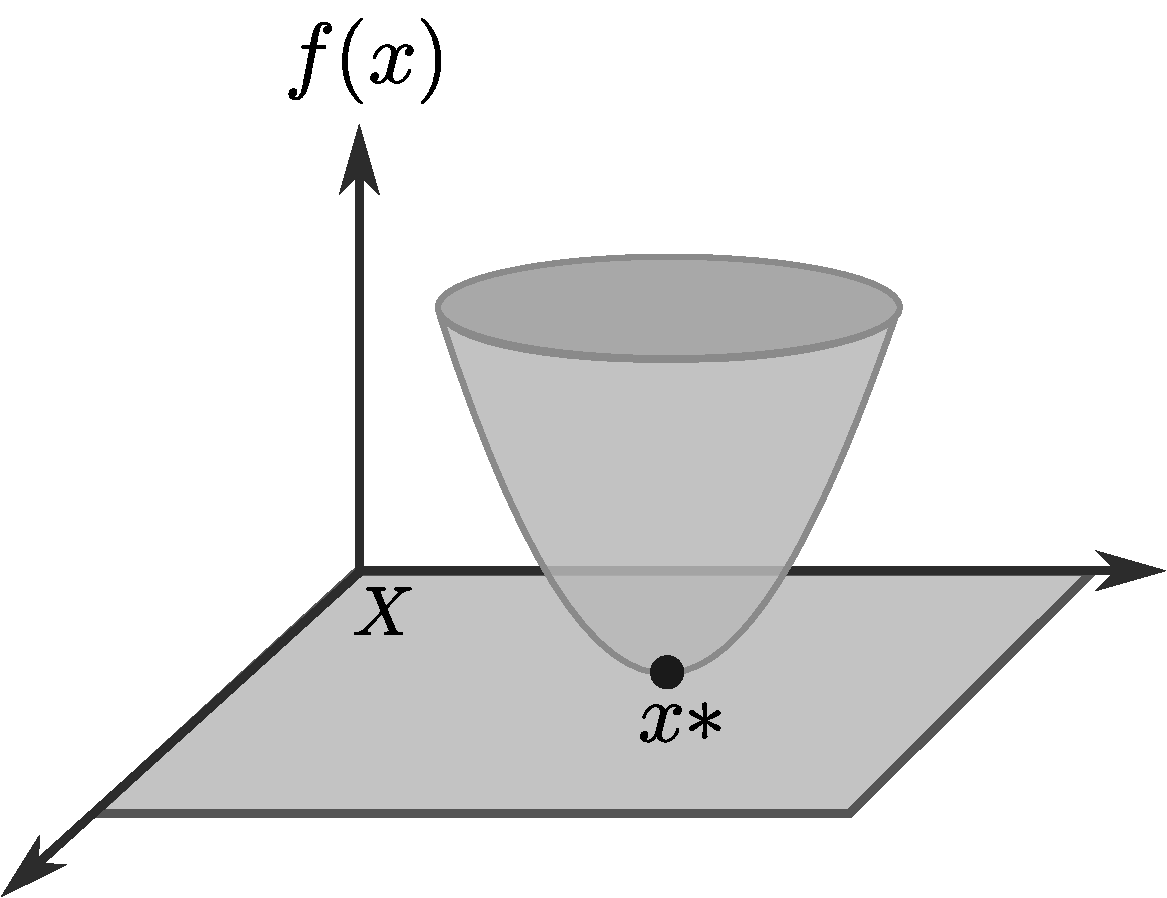
\includegraphics[width=0.5\linewidth]{img/monolevel.pdf}
    \caption{Single-objective optimization problem.}
    \label{fig:single-level}
\end{figure}

An optimization problem is solved only when a global minimum
is found. However, global minimum are, in general, difficult to find. Therefore,
in practice, we often have to find at least a local minimum \cite{rao2009engineering,back}.


After the above definitions, a general single-objective BO problem with single-objective
functions at both levels can be defined as follows \cite{bard2013practical,dempe2002foundations}:

\noindent
Minimize
\begin{equation}
    F(\vec{x},\ \vec{y}) \ \ \vec{x} \in X , \ \vec{y} \in Y 
    \label{eqn:minF1}
\end{equation}
% 
subject to:
% 
\begin{align}
    \label{eqn:y-arg}
    &\vec{y} \in \arg \min \{ f(\vec{x}, \vec{y}) \ : \ g_j(\vec{x}, \vec{y}) \leq 0, \ j = 1,\ldots, J \}\\
    &G_k(\vec{x}, \vec{y})  \leq 0, \ k = 1,\ldots,K
    \label{eqn:G}
\end{align}
where $F: X \times Y \to \mathbb{R}$ and $f: X \times Y \to \mathbb{R}$
are the upper-level objective function (leader) and lower-level objective function
(follower), respectively. In this work, $X \subseteq \mathbb{R}^n$ and
$Y \subseteq \mathbb{R}^m$ are considered. Here, $G$ and $g$ are the inequality
constraints of the upper and lower levels, respectively. Figure \ref{fig:bilevel}
shows a schematic diagram of a BO problem.
% 
\begin{figure}[!ht]
    \centering
    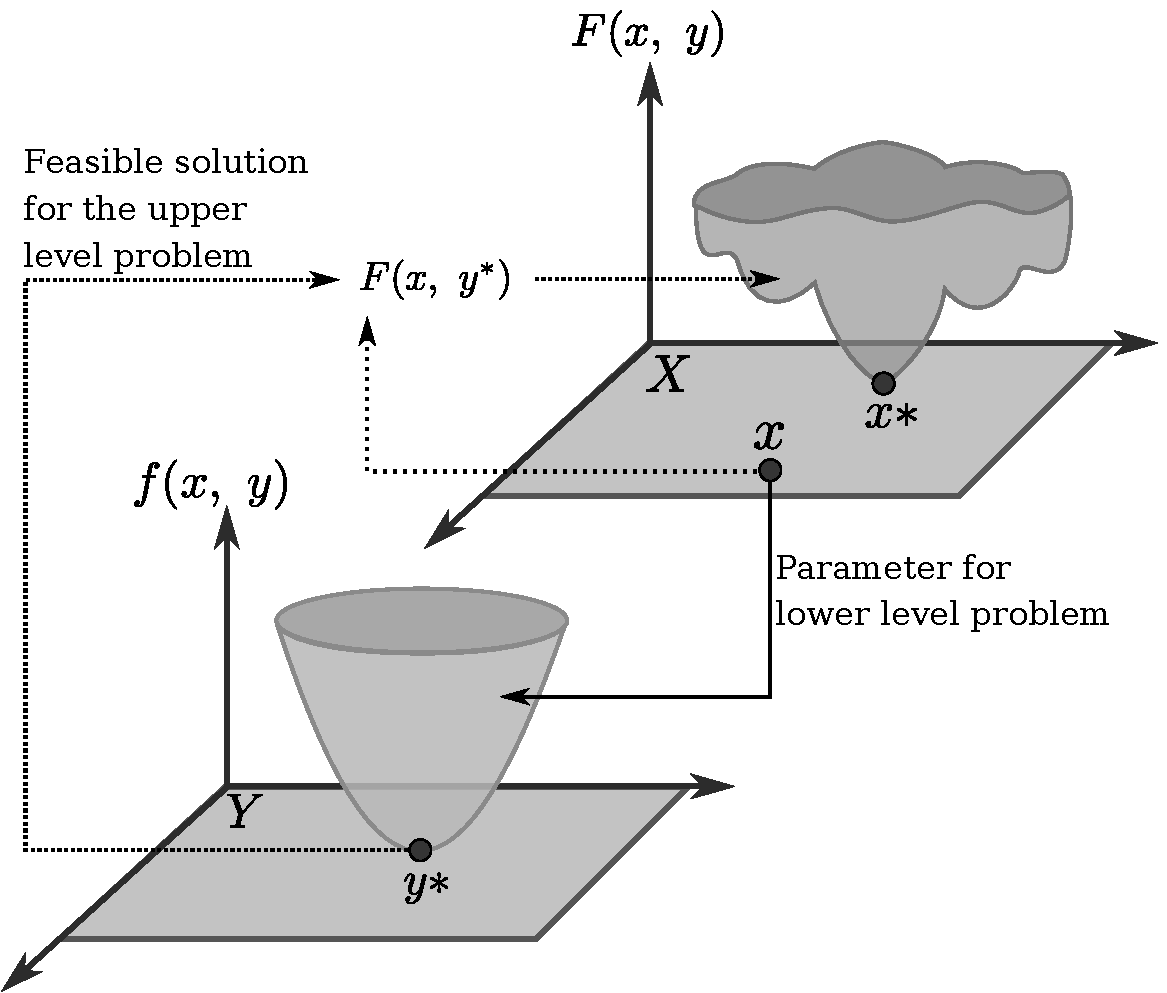
\includegraphics[width=0.8\linewidth]{img/bilevel.pdf}
    \caption{Diagram of a bilevel optimization problem. Here, $y^*$ 
            is defined as in Eq. (\ref{eqn:y-arg}). Note that $(x,\ y^*)$
            is a feasible solution.}
    \label{fig:bilevel}
\end{figure}

In 1992, Hansen et al. probed that BO problems are (strongly) NP-hard because 
evaluating a solution in the simplest BO problem (unimodal linear programming at
both levels) is also NP-hard \cite{hansen1992new,vicente1994descent}. Moreover,
many real-world problems can be naturally modeled as BO problems \cite{sinha2018review},
for example: taxation, border security problems, transportation problems, machine
learning algorithms tuning, among others \cite{bard2013practical,sinha2018review,arroyo2010bilevel}.

Due to the importance of BO, many authors have proposed different kind of solutions
for those problems e.g. mathematical approaches (mathematical programming,
Karush-Kuhn-Tucker condition for single-level reduction) \cite{dempe2002foundations,shi2005extended},
evolutionary computation (genetic algorithms, evolution strategies) and swarm
intelligence (particle swarm optimization) \cite{derrac2011practical,angelo2013differential,li2006hierarchical}.

In order to handle BO problems three strategies are identified: (1) nested,
(2) single-level reduction and (3) penalty methods. Nested strategies can be effective
but with a high computational cost when objective functions are expensive to
calculate or when high-dimensionality is present. Single-level reduction is used to
transform a BO problem into a single-level problem, usually via Karush-Kuhn-Tucker
conditions for smooth lower level objective function. As a consequence, this strategy
is restricted to differentiable functions \cite{dempe2002foundations,colson2007overview}.
Penalty methods transform a constrained method into an unconstrained optimization
problem by adding some penalties controlled by using parameters. This strategy
can be simple to understand but hard to calibrate particularly in large-scale
problems \cite{savard1994steepest,white1993penalty}.

From the literature review above mentioned, regarding population-based metaheuristics
for BO problems, most research efforts are focused on evolutionary computation and
swarm intelligence algorithms because they have been successfully applied to solve
single-level optimization problems.  On the other hand, in recent years, physics-inspired
algorithms have become popular to solve complex optimization problems and they
have provided a competitive performance when solving single-level optimization
problems \cite{fisicaSurvey}. 


This is the main motivation of this research work, where a first proposal of a
physics-inspired algorithm, originally designed for global optimization \cite{Mejia2018},
is now presented to deal with BO problems. Here, an unconstrained nested scheme
is considered.

Our approach is called Bilevel Centers Algorithm (BCA) and it is based on the center
of mass concept \cite{Mejia2018}. Without loss of generality, we assume a maximization
problem for non-negative functions $f$ and $F$ for lower and upper objective
functions, respectively. The center of mass concept is used in both levels, in
order to generate new biased directions towards promising/feasible regions of
the search space.


This paper is organized as follows: Section \ref{sec:ll-optimizer} presents the
lower level optimizer which uses the center of mass concept to promote a biased
search to promising search space regions. The proposed approach is detailed in
Section \ref{sec:bca}. After that, Section \ref{sec:experiments} shows the experimental
design and the corresponding results and discussions about the performance of the
proposed approach, where a state-of-the-art for BO optimization is used for comparison
purposes. The conclusions and future work of this research are described in
Section \ref{sec:conclu} and Section \ref{sec:future}, respectively.


%%%%%%%%%%%%%%%%%%%%%%%%%%%%%%%%%%%%%%%%%%%%%%%%%%%%%%%%%%%%%%%%%%%%%%%%
\section{Lower Level Optimizer} % (fold)
%%%%%%%%%%%%%%%%%%%%%%%%%%%%%%%%%%%%%%%%%%%%%%%%%%%%%%%%%%%%%%%%%%%%%%%%
\label{sec:ll-optimizer}

The center of mass is the unique point $\vec{c}$ at the center of a mass distribution
$U = \{\vec{u}_1,\; \vec{u}_2 , \ldots , \vec{u}_K \}$ in a space that 
has the property that the weighted sum of $K$ position vectors relative to this
point is zero \cite{Mejia2018}, as indicated in Eq. \ref{eqn:masscenter}:

\begin{equation}
    \sum_{i = 1}^K m(\vec{u}_i) (\vec{u}_i - \vec{c}) = 0,  \text{ implies } 
    %%%%%%%%%%%%%%%%%%%%%
    \vec{c} = \dfrac{1}{M} \sum_{i = 1}^K  m(\vec{u}_i)  \vec{u}_i,
    \label{eqn:masscenter}
\end{equation}
%
%
where $m(\vec{u}_i)$ is the mass of $\vec{u}_i$ and  $M$ is the sum of the 
masses of vectors in $U$. Here, $m$ is a non-negative function.
 
Thus, the lower level optimizer works as follows: for each solution $\vec{y}_i $
in the population $P = \{ \vec{y}_1,\ \vec{y}_2, \ \ldots, \ \vec{y}_{N} \} $
of $N$  solutions in $Y$, we generate $U_i \subset P $ with $K$ different
solutions such that
% 
$$
\bigcup_{i=1}^N U_i = P.
$$
%
Next, from $U_i$ the center of mass $\vec{c}_i$ is computed by using Eq. \ref{eqn:masscenter}
considering $m(\vec{u}) = f(\vec{p}, \vec{u})$, where $\vec{p}$ is given by the
upper level optimizer. After that, the worst element $\vec{u}_{\text{worst}}$
in $U_i$ is selected according to the following rule:
% 
$$
    \vec{u}_{\text{worst}} \in \arg \min \{f(\vec{p}, \ \vec{u} ) 
    % 
    \ : \
    % 
    \vec{u} \in U_i \}.
$$
% 
Now, we are able to generate a direction to locate a new solution $ \vec{q}_i$
using the already generated center of mass $\vec{c}_i$, the current solution
$\vec{y}_i$ and the worst solution $\vec{u}_{\text{worst}}$ by using Eq. \ref{eqn:vcu2}:
% 
\begin{equation}
    \vec{q}_i = \vec{y}_i + \eta _{i} ( \vec{c}_i - \vec{u}_{ \text{worst} } ) ,
    \label{eqn:vcu2}
\end{equation}
% 

Due to this stochastic strategy, this variation operator can help the exploration-exploitation 
process to avoid premature convergence because it combines the center of mass as
an attractor to promising regions of the search space but using the position of
the worst solution as a reference to get far away from it \cite{Mejia2018}. The
replacement operator works as follows: if $\vec{q}_i$ is better than $\vec{y}_i$,
then the worst element in $P$ is replaced by $\vec{q}_i$.


A linear reduction of the population size (deleting the worst elements) is applied.
The initial population size is $ N(0) = K*D$ and the final population size $N(T) =  2*K$
(for successfully generating the center of mass). Thus, the population size over
time is as in Eq. \ref{eqn:redpop}:

\begin{equation}
    N(t) = KD - \dfrac{(KD - 2K)  t}{T} 
    = K \left( D - \dfrac{(D - 2)  t}{T} \right),
\label{eqn:redpop}
\end{equation}
% 
where $t = 0,1,2,\ldots,T$ and $T$ is the maximum number of iterations.

The procedure for the implementation of the lower level optimizer is detailed in
Algorithm \ref{alg:ll-optimizer}.
% 
\begin{algorithm}[!ht]
    \caption{Lower Level Optimizer pseudocode}
    \label{alg:ll-optimizer}
    \begin{algorithmic}[1]
        \REQUIRE {upper level parameter $\vec{p}$, $K = 7, \; \eta_{\max} = 2$}
        \STATE $N \gets K*D$
        \STATE Initialize a population $P \subset Y$ with $N$ elements
        \WHILE{the end criterion is not achieved}
            \FOR {each $\vec{y}$ in $P$}
                \STATE Generate a subset $U \subset P$ with $K$ solutions
                \STATE Calculate $\vec{c}$ using $U$ with (\ref{eqn:masscenter})
                \STATE $\eta \gets \text{rand}(0,\; \eta_{\max}) $ 
                \STATE Compute $\vec{q}$ using Eq. (\ref{eqn:vcu2})
                % 
                \IF{$ f (\vec{p},\ \vec{y}) < f (\vec{p}, \ \vec{q})  $}
                    \STATE Replace worst element in $P$ with $\vec{q}$
                \ENDIF
                % 
            \ENDFOR
            % 
            \STATE Resize $P$ with Eq. \ref{eqn:redpop}
        \ENDWHILE
        \RETURN {the best solution in $P$}
    \end{algorithmic}
\end{algorithm}


% section eca (end)


%%%%%%%%%%%%%%%%%%%%%%%%%%%%%%%%%%%%%%%%%%%%%%%%%%%%%%%%%%%%%%%%%%%%%%%%
\section{BCA} % (fold)
\label{sec:bca}
%%%%%%%%%%%%%%%%%%%%%%%%%%%%%%%%%%%%%%%%%%%%%%%%%%%%%%%%%%%%%%%%%%%%%%%%

Here, BCA is presented as the upper lower level optimizer. We start describing the
variation operator of BCA and its properties. Let $F$ and $f$ be 
defined as in Eq. (\ref{eqn:minF1}) and Eq. (\ref{eqn:y-arg}), respectively.
Without loss of generality we can assume that both $F$ and $f$ are non-negative
and we want to maximize them. Hence, the population for a BO problem can be
defined as in Eq. \ref{eqn:ECApop}: 
\begin{equation}
    P = \{ (\vec{x}_1,\; \vec{y}_1), \ (\vec{x}_2,\; \vec{y}_2), \ldots,
           (\vec{x}_N,\; \vec{y}_N)
         \}
         \subset X \times Y,
        \label{eqn:ECApop}
\end{equation}
where $\vec{y}_i \in \arg \min \{ f(\vec{x}_i, \ \vec{z}) \ : \ \vec{z} \in Y \}$
for $i = 1,\ldots,N$. Here, $\vec{x}_i$ is generated at random with uniform distribution.
% 

\subsection{Algorithm Description} % (fold)
\label{sub:algorithm_description}

\begin{figure}[!ht]
    \centering
    \includegraphics[width=0.95\linewidth]{img/bca-ul.pdf}
    \caption{Diagram of BCA. Here, $x_1,\ldots,x_K$ are used to compute better
    upper level parameters $\vec{p}$. Note that $(x_i,\ y_i^*)$ and
    $(\vec{p},\ \vec{q})$ represent feasible solutions.}
    \label{fig:bca-diag}
\end{figure}

Now, we are able to describe the BCA procedure: for each iteration and each
solution $(\vec{x}_i,\; \vec{y}_i) \in P$, a new upper level parameter is generated
using the formulation in Eq. \ref{eqn:vcu2F}:
% 
\begin{equation}
    \vec{p}_i =  \vec{x}_i + \eta _{i} ( \vec{c}_i - \vec{u}_{ \text{worst} } ),
    \label{eqn:vcu2F}
\end{equation}
% 
%
where the $\vec{c}_i$ is the center of mass computed using:
%
\begin{equation}
    \vec{c}_i = \dfrac{1} {W} \sum_{(x,y) \in U} Q(\vec{x},\ \vec{y}) \cdot \vec{x} , 
            \hspace{0.5cm} 
            W = \sum_{ (x,y) \in U} Q(\vec{x},\ \vec{y}),
            % \hspace{0.5cm} 
            % U \subseteq P.
    \label{eqn:centerF}
\end{equation} 
% 
where $Q(\vec{x},\ \vec{y}) = F(\vec{x},\ \vec{y}) + f(\vec{x},\ \vec{y})$, $U \subset P $
such that card$(U) = K$  and $\vec{u}_{ \text{worst}}$ is the first coordinate of
the worst element in $U$, see Eq. \ref{eqn:uplev-worst}.

\begin{equation}
    \vec{u}_{\text{worst}} \in \arg \min \{Q(\vec{u}, \ \vec{y} ) 
    % 
    \ : \
    % 
    \vec{u} \in U_i \}
    \label{eqn:uplev-worst}
\end{equation}
% 
Note that the function $Q(\vec{x},\ \vec{y})$ is used to translate the upper level
population towards regions where $F$ is maximized while $f$ may control the bias to
feasible solutions.

Finally, the new solution is given by $ (\vec{p}, \ \vec{q}) $ which may 
replace the worst solution in $ P $ if it is better than $(\vec{x}_i,\; \vec{y}_i)$. Here,
$  \vec{q} = \arg \min _ {\vec{z} \in Y} f (\vec{p}, \ \vec{z}) $ obtained
by applying Algorithm \ref{alg:ll-optimizer}. Figure \ref{fig:bca-diag}
shows a representation of BCA solution update. 

The BCA approach requires the definition of three parameter values: $K$, $\eta_{\max}$
and the population size. Here, $K$ is useful to handle the multi-modality, i.e.,
large $K$ values provide fast convergence to local optima (useful for unimodal functions).
When $K$ takes small values, BCA favors an exploratory process. $\eta_{\max}$ mainly
controls the exploratory process as the stepsize is controlled by this parameter.
The parameter setting recommended by preliminary experiments is $K = 7$ and $\eta_{\max} = 2$.

BCA is summarized in Algorithm \ref{alg:BCA}. This proposed algorithm was used to
solve a set of eight test problems to assess the performance of BO algorithms,
known as SMD problems. Those test problems  are described
in \cite{angelo2013differential,sinha2012unconstrained,sinha2014test}.
% 
% 
% 
% 
\begin{algorithm}[!ht]
    \caption{BCA pseudocode}
    \label{alg:BCA}
    \begin{algorithmic}[1]
        % \Procedure{BCA}{$K = 7, \; \eta_{\max} = 2,\ t/T = 0.95,\ P_{\text{bin}} = 0.7$}
        \STATE $N \gets K * D$
        \STATE Generate and evaluate start population $P$ with $N$ elements
        \WHILE{the end criterion is not achieved}
            \FOR {each $(\vec{x},\; \vec{y})$ in $P$}
                \STATE Generate a subset $U \subset P$ such that  card$(U) = K$
                \STATE Calculate $\vec{c}$ using $U$ with Eq. (\ref{eqn:centerF})
                \STATE $\eta \gets \text{rand}(0,\; \eta_{\max}) $ 
                \STATE Calculate $\vec{p}$ using Eq. (\ref{eqn:vcu2F})
                \STATE Find $\displaystyle \vec{q} \in \arg \min_{\vec{z}\in Y} f(\vec{p},\ \vec{z})$ by using Algorithm \ref{alg:ll-optimizer}
                
                \IF{$ G (\vec{x},\ \vec{y}) < G (\vec{p},\ \vec{q})  $}
                    \STATE Replace worst element in $P$ with $(\vec{p},\ \vec{q})$.
                \ENDIF
            \ENDFOR
            \STATE Resize $P$ with Eq. \ref{eqn:redpop}
        \ENDWHILE
        \STATE Report best solution in $P$
        % \EndProcedure
    \end{algorithmic}
\end{algorithm}

%%%%%%%%%%%%%%%%%%%%%%%%%%%%%%%%%%%%%%%%%%%%%%%%%%%%%%%%%%%%%%%%%%%%%%%%
\section{Experiments and Discussion}
\label{sec:experiments}
%%%%%%%%%%%%%%%%%%%%%%%%%%%%%%%%%%%%%%%%%%%%%%%%%%%%%%%%%%%%%%%%%%%%%%%%

The configuration used in BCA for the experiments performed was as follows:
% 
% 
The number of Function Evaluations (NFEs) was fixed for the upper level: $500D_{UL} = 2500$, 
and the lower level: $500D_{UL}*500D_{LL} = 6,250,000$ total NFEs for both levels.
The remaining parameters were set as follows:
\begin{itemize}
    \item Upper level dimension $D_{UL} = 5$
    \item Lower level dimension $D_{LL} = 5$
    \item Upper level population size $K*D_{UL}$
    \item Lower level population size $K*D_{LL}$
    \item $K = 7$
    \item $\eta_{\max} = 2$
    \item Stop condition: BCA stopped when the accuracy ($1\times 10^{-4}$) or
    the maximum NFEs allowed was reached.
\end{itemize}


BCA was compared against BLEAQ which is a state-of-the-art evolutionary algorithm
for BO problems \cite{sinha2018review,sinha2013efficient}. BLEAQ is based on quadratic
approximations of optimal lower level variables with respect to the upper level
variables. Such strategy lets BLEAQ to reduce the NFEs having competitive results.
BLEAQ was run with the parameters suggested by the authors \cite{sinha2018review,sinha2013efficient}
and the stop criteria was maintained but accuracy was set at $1\times 10^{-4}$ as
in BCA. Both algorithms were used to solve independently 31 times each test problem.



\begin{table}[!ht]
\renewcommand{\arraystretch}{1.3}
    \caption{Upper level accuracy statistics by BCA obtained from 31 independent runs.}
    \label{tab:ul-accuracy}
    \centering
    \begin{tabular}{|c|c|c|c|c|c|c|}
%---------------------------------------------
\hline
&\textbf{Best}&\textbf{Median}&\textbf{Mean}&\textbf{Worst}&\textbf{Std.}\\ \hline 
%---------------------------------------------
\textbf{SMD1} & 1.51E--05 & 5.35E--05 & 5.28E--05 & 8.34E--05 & 1.90E--05 \\ \hline 
\textbf{SMD2} & 1.50E--05 & 4.68E--05 & 5.88E--05 & 3.11E--04 & 5.13E--05 \\ \hline 
\textbf{SMD3} & 1.57E--05 & 5.51E--05 & 2.40E--04 & 3.54E--03 & 6.60E--04 \\ \hline 
\textbf{SMD4} & 4.09E--08 & 4.90E--05 & 6.20E--05 & 3.01E--04 & 6.70E--05 \\ \hline 
\textbf{SMD5} & 2.30E--05 & 5.03E--05 & 4.78E--05 & 8.33E--05 & 1.74E--05 \\ \hline 
\textbf{SMD6} & 1.57E--01 &  1.90E+01 &  2.59E+01 &  1.40E+02 &  2.95E+01 \\ \hline 
\textbf{SMD7} & 9.34E--01 & 9.75E--01 &  1.19E+00 &  3.81E+00 & 6.00E--01 \\ \hline 
\textbf{SMD8} & 1.58E--05 & 6.49E--05 & 1.83E--04 & 2.23E--03 & 4.11E--04 \\ \hline 
%---------------------------------------------
    \end{tabular}
\end{table}

\begin{table}[!ht]
\renewcommand{\arraystretch}{1.3}
    \caption{Lower level accuracy statistics by BCA obtained from 31 independent runs.}
    \label{tab:ll-accuracy}
    \centering
    \begin{tabular}{|c|c|c|c|c|c|c|}
%---------------------------------------------
\hline
&\textbf{Best}&\textbf{Median}&\textbf{Mean}&\textbf{Worst}&\textbf{Std.}\\ \hline 
%---------------------------------------------
\textbf{SMD1} & 2.67E--06 & 2.06E--05 & 2.14E--05 & 4.75E--05 & 9.77E--06 \\ \hline 
\textbf{SMD2} & 3.56E--06 & 1.81E--05 & 2.07E--05 & 4.60E--05 & 1.15E--05 \\ \hline 
\textbf{SMD3} & 1.87E--07 & 2.24E--05 & 3.12E--04 & 4.31E--03 & 9.28E--04 \\ \hline 
\textbf{SMD4} & 6.23E--06 & 3.65E--05 & 1.53E--04 & 7.96E--04 & 2.33E--04 \\ \hline 
\textbf{SMD5} & 2.50E--06 & 2.01E--05 & 2.19E--05 & 4.55E--05 & 1.28E--05 \\ \hline 
\textbf{SMD6} & 3.91E--04 & 2.86E--02 & 4.23E--02 & 1.84E--01 & 4.35E--02 \\ \hline 
\textbf{SMD7} &  3.71E+02 &  3.74E+02 &  3.74E+02 &  3.75E+02 &  1.01E+00 \\ \hline 
\textbf{SMD8} & 1.18E--06 & 2.33E--05 & 6.53E--05 & 7.93E--04 & 1.44E--04 \\ \hline 

%---------------------------------------------
    \end{tabular}
\end{table}

\begin{table}[!ht]
\renewcommand{\arraystretch}{1.3}
    \caption{Upper level NFEs statistics by BCA obtained from 31 independent runs.}
    \label{tab:ul-fes}
    \centering
    \begin{tabular}{|c|c|c|c|c|c|c|}
%---------------------------------------------
\hline
&\textbf{Best}&\textbf{Median}&\textbf{Mean}&\textbf{Worst}&\textbf{Std.}\\ \hline 
%---------------------------------------------
\textbf{SMD1} & 1244 & 1526 & 1539.42 & 1879 & 152.119 \\ \hline
\textbf{SMD2} & 1244 & 1481 & 1482.84 & 2501 & 220.7   \\ \hline
\textbf{SMD3} & 1365 & 1526 & 1647.84 & 2501 & 287.517 \\ \hline
\textbf{SMD4} & 1169 & 1435 & 1437.26 & 1800 & 131.393 \\ \hline
\textbf{SMD5} & 1317 & 1526 & 1554.42 & 1898 & 137.766 \\ \hline
\textbf{SMD6} & 2501 & 2501 & 2501 &  2501 &   0   \\ \hline
\textbf{SMD7} & 2501 & 2501 & 2501 &  2501 &   0   \\ \hline
\textbf{SMD8} & 1780 & 2219 & 2234.65 & 2501 & 206.959 \\ \hline


%---------------------------------------------
    \end{tabular}
\end{table}

\begin{table}[!ht]
\renewcommand{\arraystretch}{1.3}
    \caption{Lower level NFEs statistics by BCA obtained from 31 independent runs.}
    \label{tab:ll-fes}
    \centering
    \begin{tabular}{|c|c|c|c|c|c|c|}
%---------------------------------------------
\hline
&\textbf{Best}&\textbf{Median}&\textbf{Mean}&\textbf{Worst}&\textbf{Std.}\\ \hline 
%---------------------------------------------
\textbf{SMD1} & 3110000  & 3815000  & 3848548.4  & 4697500  & 380298.6 \\ \hline
\textbf{SMD2} & 3110000  & 3702500  & 3707096.8  & 6252500  & 551750.7 \\ \hline
\textbf{SMD3} & 3412500  & 3815000  & 4119596.8  & 6252500  & 718793.3 \\ \hline
\textbf{SMD4} & 2922500  & 3587500  & 3593145.2  & 4500000  & 328481.3 \\ \hline
\textbf{SMD5} & 3292500  & 3815000  & 3886048.4  & 4745000  & 344415.4 \\ \hline
\textbf{SMD6} & 6252500  & 6252500  & 6252500  & 6252500  & 0 \\ \hline
\textbf{SMD7} & 6252500  & 6252500  & 6252500  & 6252500  & 0 \\ \hline
\textbf{SMD8} & 4450000  & 5547500  & 5586612.9  & 6252500  & 517397.6 \\ \hline
%---------------------------------------------
    \end{tabular}
\end{table}

% %%%%%%%%%%%%%%%%%%%%%%%%%%%%%%%%%%%%%%%%%%%%%%%%%%%%%
% %%%%%%%%%%%%%%%%%%%%%%%%%%%%%%%%%%%%%%%%%%%%%%%%%%%%%

\begin{table}[!ht]
\renewcommand{\arraystretch}{1.3}
    \caption{Median NFEs values by BCA and BLEAQ obtained from 31 independent runs.}
    \label{tab:ul-comparative-fes}
    \centering
    \begin{tabular}{|c|c|c||c|c|}
%---------------------------------------------
\hline
& \multicolumn{2}{c||}{Upper Level} & \multicolumn{2}{c|}{Lower Level} \\ \hline
& BCA & BLEAQ & BCA & BLEAQ \\ \hline
%---------------------------------------------
 % & bca.ul & bleaq.ul & bca.ll & bleaq.ll \\ \hline
SMD1 & \textbf{1526} & 1600 & 3815000 & \textbf{116088} \\ \hline
SMD2 & \textbf{1481} & 1925 & 3702500 & \textbf{113504} \\ \hline
SMD3 & \textbf{1526} & 1630 & 3815000 & \textbf{122542} \\ \hline
SMD4 & \textbf{1435} & 1750 & 3587500 & \textbf{70906} \\ \hline
SMD5 & \textbf{1526} & 3031 & 3815000 & \textbf{147289} \\ \hline
SMD6 &     2501      & \textbf{1016} & 6252500 & \textbf{7055} \\ \hline
SMD7 &     2501      & \textbf{2104} & 6252500 & \textbf{130195} \\ \hline
SMD8 & \textbf{2219} & 5569 & 5547500 & \textbf{289886} \\ \hline
%---------------------------------------------
    \end{tabular}
\end{table}

% %%%%%%%%%%%%%%%%%%%%%%%%%%%%%%%%%%%%%%%%%%%%%%%%%%%%%
\begin{table}[!ht]
\renewcommand{\arraystretch}{1.3}
    \caption{Median accuracy values by BCA and BLEAQ obtained from 31 independent runs.}
    \label{tab:ll-comparative-vals}
    \centering
    \begin{tabular}{|c|c|c||c|c|}
%---------------------------------------------
\hline
& \multicolumn{2}{c||}{Upper Level} & \multicolumn{2}{c|}{Lower Level} \\ \hline
& BCA & BLEAQ & BCA & BLEAQ \\ \hline
%---------------------------------------------
SMD1  & \textbf{5.35E--05} &          9.91E--05 & \textbf{2.06E--05} &          6.72E--05 \\ \hline
SMD2  & \textbf{4.68E--05} &          2.82E--04 & \textbf{1.81E--05} &          3.84E--04 \\ \hline
SMD3  &          5.51E--05 & \textbf{4.96E--06} &          2.24E--05 & \textbf{6.26E--06} \\ \hline
SMD4  & \textbf{4.90E--05} &          1.54E--04 & \textbf{3.65E--05} &          6.12E--04 \\ \hline
SMD5  & \textbf{5.03E--05} &          1.62E--04 & \textbf{2.01E--05} &          3.08E--04 \\ \hline
SMD6  &           1.90E+01 & \textbf{1.46E--13} &          2.86E--02 & \textbf{8.66E--16} \\ \hline
SMD7  &          9.75E--01 & \textbf{9.76E--02} &           3.74E+02 &  \textbf{1.25E+02} \\ \hline
SMD8  & \textbf{6.49E--05} &          7.46E--03 & \textbf{2.33E--05} &          5.63E--03 \\ \hline

%---------------------------------------------
    \end{tabular}
\end{table}






Tables \ref{tab:ul-accuracy} and \ref{tab:ll-accuracy} show the statistical results
of the accuracy values obtained by the proposed BCA in the two levels of each BO
test problem. Moreover, the best, median, mean, worst and standard deviation values
of the NFEs required to solve each BO test problem using BCA are given in
Table \ref{tab:ul-fes} and \ref{tab:ll-fes} for each level, respectively. 
Tables \ref{tab:ul-comparative-fes} and \ref{tab:ll-comparative-vals} compare the
median accuracy and NFEs at the upper and lower levels required by BCA against
those values obtained by BLEAQ. A result in boldface indicates the best value found.

From Tables \ref{tab:ul-accuracy} and \ref{tab:ll-accuracy} it can be observed
that BCA is able to consistently reach very competitive results in all test problems
for both levels. Just problem SMD7 was difficult to solve by BCA. 

A similar robust performance was observed by BCA in the upper level regarding NFEs
as indicated in Table \ref{tab:ul-fes}. In contrast, more variation in the number
of NFEs was reported in Table \ref{tab:ll-fes} for the lower level. 



Regarding the comparison against the state-of-the-art algorithm, from Table \ref{tab:ll-comparative-vals}
it can be concluded that BCA outperformed BLEAQ in five BO test problems in the
upper level and also in five BO test problems in the lower level. Furthermore,
BCA required less NFEs in the upper level of six BO test problems based on
Table \ref{tab:ul-comparative-fes}. However, BLEAQ clearly outperformed BCA in
the number of lower level NFEs as indicated in the same Table \ref{tab:ul-comparative-fes}.

Note that no statistical test was used to compare the algorithms, since the
obtained values (from the objective functions) may not represent feasible solutions
and that can be an unfair comparison of the performance of the algorithms.



%%%%%%%%%%%%%%%%%%%%%%%%%%%%%%%%%%%%%%%%%%%%%%%%%%%%%%%%%%%%%%%%%%%%%%%%
\section{Conclusions}
\label{sec:conclu}
%%%%%%%%%%%%%%%%%%%%%%%%%%%%%%%%%%%%%%%%%%%%%%%%%%%%%%%%%%%%%%%%%%%%%%%%

This work presented the adaptation of a physics-inspired algorithm based on the
center of mass (BCA) to solve bilevel optimization problems. Both levels used a
similar variation operator based on the center of mass to find promising regions
of the search space and a greedy replacement based on fitness. BCA is a simple
algorithm which requires just three parameters to be fine-tuned by the user (the
population size, the size of the subset to compute the center of mass and the
stepsize for the variation operator). Eight test problems were solved to assess
the performance of the proposed algorithm in terms of upper/lower level accuracy
and function evaluations compared against a state-of-the-art evolutionary algorithm
for BO. The overall results suggest that BCA was able to provide competitive
results in terms of accuracy compared to those obtained by BLEAQ even requiring
less evaluations in the upper level. However BLEAQ outperformed BCA with respect
to the number of evaluations required at the lower level.


%%%%%%%%%%%%%%%%%%%%%%%%%%%%%%%%%%%%%%%%%%%%%%%%%%%%%%%%%%%%%%%%%%%%%%%%
\section{Future Work}
\label{sec:future}

The future paths of research are the following: carry out a study in
order to approximate feasible solutions at the lower level to decrease number of
evaluations required and explore some penalty methods to transform the
nested scheme into a single level optimization problem. Study or propose a technique
to compare the algorithm performance for bilevel optimization problems.
%%%%%%%%%%%%%%%%%%%%%%%%%%%%%%%%%%%%%%%%%%%%%%%%%%%%%%%%%%%%%%%%%%%%%%%%

\section*{Acknowledgments}
The first author acknowledges support from the Mexican Council for Science and
Technology (CONACyT) for a scholarship to pursue graduate studies at the University
of Veracruz. The second author acknowledges support from CONACyT through project
No. 220522. 





% trigger a \newpage just before the given reference
% number - used to balance the columns on the last page
% adjust value as needed - may need to be readjusted if
% the document is modified later
%\IEEEtriggeratref{8}
% The "triggered" command can be changed if desired:
%\IEEEtriggercmd{\enlargethispage{-5in}}

\bibliographystyle{IEEEtran}
\bibliography{IEEEabrv,../../../conf/references,../../../conf/references-bilevel}



% that's all folks
\end{document}



